\documentclass[../../main.tex]{subfiles}

\begin{document}

At the time the Wedge paper was published, ciphers that offer forward
secrecy were not common place; hence, the authors of Wedge deemed it
unnecessary to provide support for this category of ciphers. However,
forward secrecy has gained popularity since, with
[STATISTIC][CITATION]. We have, therefore, designed our system to
accomodate ciphers within this category. As of TLSv1.2 ciphers that
offer forward secrecy employ some variant of Diffie-Hellman (DH) Key
Exchange to establish the \texttt{PremasterSecret}. Before discussing
the SSL/TLS handsake for these ciphers, we provide a brief
explaination of DH Key Exchange.


DH Key Exchange is an asymmetric cryptographic algorithm used to
arrive at a shared secret between two parties. DH Key Exchange can be
best illustrated using the famous ``paint mixing'' analogy. The
analogy is presented in Figure~\ref{fig:paint}.
\begin{enumerate}
  \item The partiticpants agree to using a publicly known ``paint
    color''
  \item Each participant generates a secret ``paint color''
  \item Each participant ``mixes'' their ``secret color'' with the
    ``public color'' they previously agreed to use
  \item The participants \textit{exchange} the ``paint mixtures'' from
    the previous step
  \item The participants combine the ``paint mixture'' they received
    with their own ``secret paint''. Both parties now possess the same
    ``shared secret paint''.
\end{enumerate}
The security of DH Key Exchange relies on the assumption that it is
computationally difficult to seperate the ``paint mixtures''.
\begin{figure}[H]
  \centering
  
  \caption{DH Key Exchange paint analogy}
  \label{fig:paint}
\end{figure}
Moreover, by creating new ``secret paints'' for each session and
purging all the ``paints'' from memory after a session is complete,
one obtains Ephemeral DH Key Exchange (DHE). DHE offers forward
secrecy because no long-term private secret is used to negotiate the
shared secret; hence, compromising a single session's ``secret
paints'' does not affect any other session (new ``secret paints'' are
used for new sessions).

For our project, we concentrated on Elliptical Curves DHE (ECDHE).
This is a variant of DHE that utilises Elliptical Curves to ``mix''
the ``paints''. The mathematics behind ECDHE is beyond the scope of
this report, but the interested reader may refer to [CITATION] for
further details. The steps in the SSL/TLS handshake when using an
ECDHE cipher (``ECDHE handshake'') are presented in
Figure~\ref{fig:ecdhe-pristine}.

\begin{figure}[H]
  \centering
  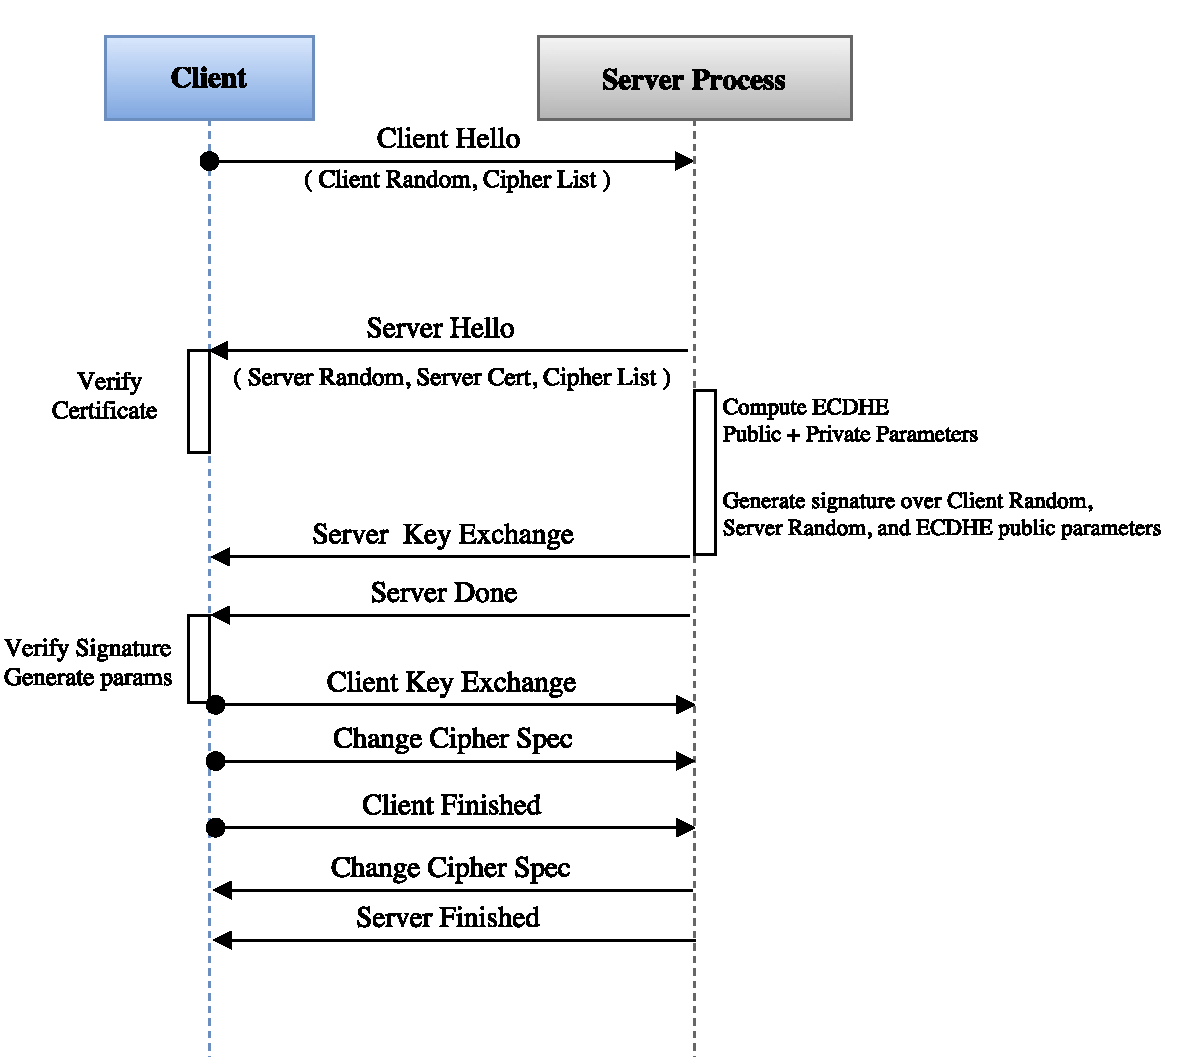
\includegraphics[scale=0.4]{images/EC-DHE-Handshake-pristine.pdf}
  \caption[``ECDHE handshake'']{SSL/TLS handshake when using an ECDHE
    cipher}
  \label{fig:ecdhe-pristine}
\end{figure}

Similair to the ``RSA handshake'', the ``ECDHE handshake'' begins by
establishing the values for \crandom~and \srandom. In performing this
exchange, the involved parties also agree on the Elliptic Curve
(``well-known paint'') to be used in negotiating the shared secret.
Following that, the server computes its private parameter (``secret
paint'') and the corresponding public parameter (``paint mixture''). A
hash function is applied across the public parameter, \srandom, and
\crandom. This resulting message digest is signed using the long-term
private key and is sent to the client, attached to the public
parameter. The client verifies the signature received, computes their
own private and public parameters, and sends the public parameter to
the server. The client and server may now derive the
\texttt{PremasterSecret}, \texttt{MasterSecret}, and the session key
block. The handshake now proceeds in the same way as the ``RSA
handshake''.

Clearly, from the discussion above, the long-term private key is used
only for verification purposes in the ``ECDHE handshake''. 




%-------------------------------------------------------------------

We have partitioned the standard EC-DHE handshake implementation in
Libressl and separated it into two components. One network facing
component is deemed untrusted and is running as a part of nginx web
server process. The other part resides inside the trusted SGX enclave
and runs as an independent process. Both the components of the server
communicate via a list of fine grained API’s
wrapped over a named pipe IPC interface.

The handshake process is carried out in two different phases, one to
authenticate the server identity and other to establish the pre master
secret. Figure~\ref{fig:ecdhe_handshake}) illustrates the messages
exchanges between client and server’s trusted and untrusted compartments.

A Https client can initiate the handshake by sending a “client hello”
enclosed with a random number and a list of Elliptic curves it
supports. Upon receiving this request, the nginx server initialises a
new session in the enclave (TODO: Add info related to session
cache/resumption.?) and configures the random number received from the
client. The server random seed is generated inside the enclave. This
will accord to additional security to the system by preventing an
adversary from exploiting the untrusted component of the server and by
influencing a session key generation based on random seeds of his
choice. Enclave code maintains separate state for each session and
will not accept server random as an input argument in any API
interfaces. After obtaining the server random, it is sent to the
client as part of the “Server Hello” message together with Server
Public key certificate and a list of server preferred ciphers.

\begin{figure}[H]
  \centering
  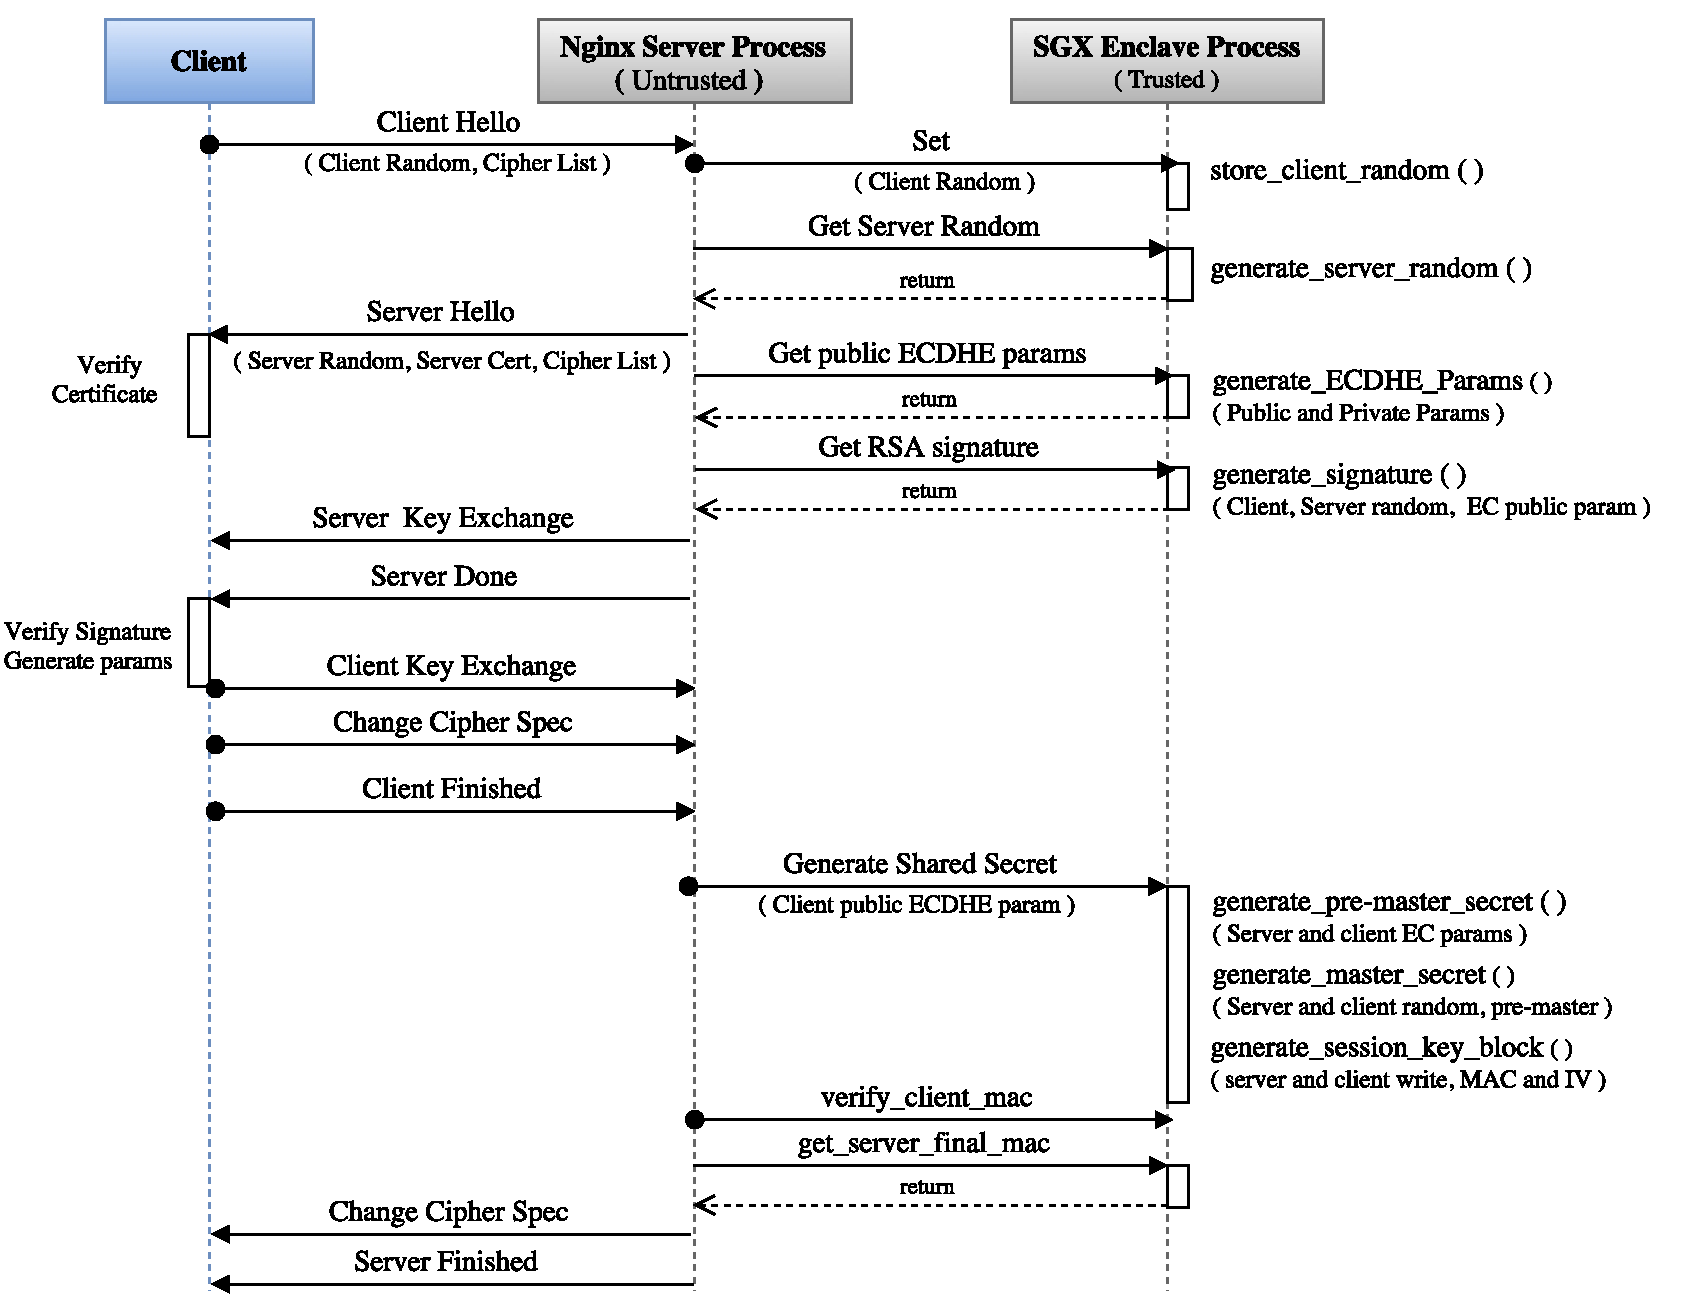
\includegraphics[scale=0.4]{EC-DHE-Handshake.pdf}
  \caption{EC-DHE Handshake}
  \label{fig:ecdhe_handshake}
\end{figure}

In the second phase of DH key exchange, the server will pick one of
the client supported elliptic curves and send the curve id to the
enclave. In the enclave we will generate both the public and private
part of the EC-DH parameters based on the chosen curve id. Only the
public part of the DH param is exposed to the nginx server process and
the private part is kept secret within the enclave. This ensures
additional security to the system by making the enclave completely
abstain from accepting any server side seeds pertaining the shared
secret generation.

In order to prove, that the server has control of the private key and
DH params, the Server has to produce a digital signature. In our
design this is computed within the enclave. This will include Client
Random, Server Random and Public DH Params signed using server private
key. Server sends the ECDHE parameter (in clear) together with
Signature to the client as part of the “Server Key Exchange” message.
Client verifies this message using the server public key. If the
verification is successful , the client generates its part of EC
params and sends it to the server as part of “Client Key Exchange”
message.


After receiving the “Client Key Exchange” message, the server will
attain all the required seeds to launch the shared key generation
process. The keys are calculated in a three level process. First a
Pre-Master key is computed from Client Public ECDHE param and Server
ECDHE params(both Private and Public). The pre-master is then used as
one of the seed along with Client Random and Server Random for the
shared Master secret generation. Server will finally generate the
symmetric session keys with the associated MACs and Initialisation
vectors from the master secret. All the three steps of key
generation processes is securely performed within the enclave.

The client will then send a “Change Cipher Spec” message to indicate
it will use the newly generated keys to hash and encrypt further
messages. The handshake is complete from the client end after sending
a “Finished” message containing a hash and MAC over all the previous
handshake messages. Upon receiving client finished, the server will
decrypt it using the session keys and validate the integrity of the
handshake process. If the decryption or verification fails, the
handshake is deemed to be failed and all the allocated session
resources are freed. If successful, the server sends a “Change Cipher
Spec” message indicating all messages send from now on will be
encrypted using the shared session secret keys. Finally server
computes its authenticated and encrypted “Finished” Message and sends
it to the Client. This completes the full Handshake process.

Observe, however, that \texttt{MasterSecret} is used to compute the
session key block in the untrusted component; hence, an adversary,
after exploiting the untrusted component, may leak the session key
block (or leak \texttt{MasterSecret} and derive the session key block
themselves).

\end{document}

%%% Local Variables:
%%% mode: latex
%%% TeX-master: "../../main"
%%% End:
